%% background — words; trees of arity n with variance c, normalization and
%% duality, tree classes; flat systems, signed systems, existential entailment,
%% flattening; the results of Zhao26 on constraints; readers, holes, the
%% rejected-path property, the canonical hierarchy, the tail, depth and search
%% theorems of Zhao26, lettered monitors, derivatives and the label facts, and
%% an outline of the search. Further results of Zhao26 are in app:bg.

\section{Background}\label{sec:bg}

Throughout the paper we fix an arity $n\ge0$ and a variance $c$ of the
constructor $f$. This section fixes the notation for words, trees, and
constraints, defines existential entailment, and states the results that we
use from the decidability proof for plain entailment of \citet{Zhao26}. That
paper treats one constructor of every arity and every variance; we cite its
results in that generality. Short proofs are repeated; all other cited results
are stated exactly and proved there. \Cref{app:bg} collects the further
results of that paper used later: the satisfiability criteria, the cores lemma, the ordinary
and symbolic states of derived monitors, the structure of the bounded-depth
search, and its constants.

\subsection{Words}\label{sec:bg-words}
Put $\Sigma=\{0,\ldots,n-1\}$, the alphabet of \emph{directions}; the letter
$i$ names the $i$th argument of $f$. For $n=0$ the alphabet is empty and $\eps$
is the only word over it. Readers (\cref{sec:bg-readers}) also work over other
finite alphabets, written $\Gamma$, for instance $\Sigma\sqcup\{\sep\}$.

Words are finite unless they are explicitly called infinite. For a word $w$, a
\emph{cut} is an integer $j$ with $0\le j\le\len w$; it separates the first $j$
letters from the rest. We write $w[i]$ for the letter at position $i$, where
$0\le i<\len w$, and $\wpre wj$, $\wsub wjh$, and $\wsuf wj$ for the prefix,
factor, and suffix at the indicated cuts. The empty word is $\eps$, and
$u\pre w$ means that $u$ is a prefix of $w$. For a set $L$ of words and a word
$\beta$, put $\beta L=\{\beta\sigma:\sigma\in L\}$ and
$\beta^{-1}L=\{\sigma:\beta\sigma\in L\}$. A positive integer $\varpi$ is a
\emph{period} of $w$ if $w[i]=w[i-\varpi]$ for $\varpi\le i<\len w$. For a
nonempty word $o$, we write $\theta\pre o^\omega$ if $\theta\pre o^k$ for some
$k\ge0$.

\begin{lemma}[Periodic prefixes {\nssecite{Lemma ``Periodic prefixes''}}]\label{lem:bg-periodic}
For every nonempty word $o$ and every word $\theta$, $\theta\pre o\theta$ iff
$\theta\pre o^\omega$.
\end{lemma}
\begin{proof}
If $\theta\pre o^k$, then $o\theta\pre o^{k+1}$ and $\theta\pre o^{k+1}$; of
two prefixes of one word the shorter is a prefix of the longer, so
$\theta\pre o\theta$. Conversely, let $\theta\pre o\theta$. If
$\len\theta\le\len o$, then $\theta\pre o$. Otherwise $\theta=o\theta'$ for a
word $\theta'$, and $o\theta'\pre oo\theta'$ gives $\theta'\pre o\theta'$. By
induction on the length, $\theta'\pre o^k$ for some $k$, so
$\theta\pre o^{k+1}$.
\end{proof}

\subsection{Trees, Variance, and Normalization}\label{sec:bg-trees}

\paragraph{Trees}
Order the labels by $\Bot<f<\Top$. A \emph{tree} is a partial map
$t:\Sigma^*\rightharpoonup\BFT$ whose domain $\operatorname{dom}(t)$ contains
$\eps$, is prefix closed, and satisfies, for every $w\in\operatorname{dom}(t)$
and every $i\in\Sigma$,
\[
 wi\in\operatorname{dom}(t)\quad\Longleftrightarrow\quad t(w)=f .
\]
The elements of $\operatorname{dom}(t)$ are the \emph{positions} of $t$. We
write $f(t_0,\ldots,t_{n-1})$, or $f(t_i)_i$, for the tree with root label $f$
and subtrees $t_i$ at the positions $i$. The \emph{subtree} of $t$ at a
position $\beta$ is the tree $\beta^{-1}t:w\mapsto t(\beta w)$. The full
constructor tree $\Omega=f(\Omega,\ldots,\Omega)$ has label $f$ at every word;
it is infinite for $n\ge1$, and $\Omega=f()$ for $n=0$. At arity zero the only
trees are $\Bot$, $f()$, and $\Top$.

\paragraph{Variance and the order}
A \emph{variance} is a map $c:\Sigma\to\{0,1\}$; argument $i$ is
\emph{covariant} if $c(i)=0$ and \emph{contravariant} if $c(i)=1$, and $f$ is
covariant if $c=0$. For the arrow, $n=2$, $f(a_0,a_1)=a_0\to a_1$, $c(0)=1$, and
$c(1)=0$. The \emph{polarity} of a word counts its contravariant letters modulo
two:
\begin{equation}\label{eq:bg-polarity}
 \parity(w)=\bigoplus_{j<\len w}c(w[j]),\qquad \parity(\eps)=0,\qquad
 \parity(uv)=\parity(u)\oplus\parity(v).
\end{equation}
The \emph{non-structural order} of variance $c$ is
\begin{equation}\label{eq:bg-order}
 t\le_c u\quad\Longleftrightarrow\quad
 \forall w\in\operatorname{dom}(t)\cap\operatorname{dom}(u)\quad
 \begin{cases}t(w)\le u(w),&\parity(w)=0,\\ u(w)\le t(w),&\parity(w)=1.\end{cases}
\end{equation}
For the covariant variance $c=0$ we write $\le$ and call the order
\emph{covariant}. The relation $\le_c$ is a partial order, and it is the
greatest relation $R$ such that $R(t,u)$ implies $t=\Bot$, or $u=\Top$, or
$t=f(a_i)_i$ and $u=f(b_i)_i$ with $R(a_i,b_i)$ for every $i$ with $c(i)=0$ and
$R(b_i,a_i)$ for every $i$ with $c(i)=1$
\nssecite{Sect.\ ``Non-Structural Subtyping''}. In particular,
$\Bot\le_c t\le_c\Top$ for every tree $t$, and
$f(a_i)_i\le_c f(b_i)_i$ iff each pair of arguments is related in the direction
given by its variance. For the arrow this is the usual rule:
$a_0\to a_1\le_c b_0\to b_1$ iff $b_0\le_c a_0$ and $a_1\le_c b_1$.

\paragraph{Duality and normalization}
The \emph{dual} $t^{\partial}$ of a tree $t$ has the domain of $t$ and the labels of
$t$ with $\Bot$ and $\Top$ exchanged; labels $f$ are unchanged. For a
\emph{sign} $s\in\{0,1\}$, the \emph{normalization} $\nu_s t$ has the domain of
$t$; its label at a position $w$ is that of $t$ with $\Bot$ and $\Top$ exchanged
if $s\oplus\parity(w)=1$, and unchanged otherwise. Thus $\nu_0$ exchanges the
extreme labels at the positions of odd polarity and $\nu_1$ at those of even
polarity. The polarity is taken at actual positions of $t$ only; a leaf is
never followed by further letters. For covariant $f$, $\nu_0t=t$ and
$\nu_1t=t^{\partial}$. We also write $+$ for the sign $0$ and $-$ for the sign $1$.

\begin{lemma}[Normalization {\nssecite{Lemma ``Normalization''}}]\label{lem:bg-normalization}
For every variance $c$, all trees $t,u,t_0,\ldots,t_{n-1}$, and every sign $s$:
\begin{enumerate}[leftmargin=*]
\item $\nu_s f(t_i)_i=f(\nu_{s\oplus c(i)}t_i)_i$,\quad
  $\nu_1t=(\nu_0t)^{\partial}=\nu_0(t^{\partial})$,\quad and\quad $\nu_s\nu_st=t$;
\item $t\le_c u$ iff $\nu_0t\le\nu_0u$ iff $\nu_1u\le\nu_1t$;
\item for the covariant order, $t\le u$ iff $u^{\partial}\le t^{\partial}$;
\item the subtree of $\nu_st$ at a position $w$ is $\nu_{s\oplus\parity(w)}(w^{-1}t)$,
  and $\nu_s$ and duality preserve domains, finiteness, and regularity.
\end{enumerate}
\end{lemma}
\begin{proof}
(1) The root of $f(t_i)_i$ is labeled $f$ and is never changed. At a position
$iw$ we have $\parity(iw)=c(i)\oplus\parity(w)$, so the condition $s\oplus\parity(iw)=1$
for $\nu_s$ at $iw$ is the condition for $\nu_{s\oplus c(i)}$ at the position $w$
of $t_i$. The conditions of $\nu_0$ and $\nu_1$ at a position are
complementary, so $\nu_1t$ is $\nu_0t$ with every extreme label exchanged, and
exchanging all extreme labels commutes with exchanging some of them. Applying
$\nu_s$ twice exchanges the same labels twice.

(3) Exchanging $\Bot$ and $\Top$ reverses the chain $\Bot<f<\Top$, and $t$ and
$t^{\partial}$ have the same domain, so every comparison in \cref{eq:bg-order},
read covariantly, is reversed.

(2) The trees $t$ and $\nu_0t$ have the same domain. At a common position $w$
with $\parity(w)=0$, $\nu_0$ changes neither label; at one with $\parity(w)=1$ it
applies the order-reversing exchange to both labels, so $u(w)\le t(w)$ iff
$(\nu_0t)(w)\le(\nu_0u)(w)$. Hence \cref{eq:bg-order} for $\le_c$ is the
covariant comparison of $\nu_0t$ and $\nu_0u$ at every common position. The
second equivalence follows from (1) and (3) for the covariant order.

(4) The first assertion follows from (1) by induction on $w$. So the subtrees
of $\nu_st$ are among the trees $\nu_0t'$ and $\nu_1t'$ for subtrees $t'$ of
$t$, which are finitely many if $t$ is regular. Domains are preserved by
definition, and duality is handled in the same way.
\end{proof}

Thus $\nu_0$ is an order isomorphism from the trees ordered by $\le_c$ onto the
trees ordered covariantly, and $\nu_1$ is an order anti-isomorphism. This is
how variance is removed: a constraint of variance $c$ about $t$ becomes a pair
of covariant constraints about $\nu_0t$ and $\nu_1t$
(\cref{lem:bg-signed}).

\paragraph{Tree classes}
We consider three \emph{tree classes}: the class $\Trees$ of all trees,
possibly infinite; the class $\Trees_{\mathrm{reg}}$ of \emph{regular} trees,
which have finitely many distinct subtrees; and the class $\Trees_{\mathrm{fin}}$
of \emph{finite} trees, which have finite domain. Then
$\Trees_{\mathrm{fin}}\subseteq\Trees_{\mathrm{reg}}\subseteq\Trees$, and
$\Omega$ is regular but not finite for $n\ge1$. A tree is regular iff it is the
unfolding of a finite graph whose constructor nodes have $n$ ordered successors
\nssecite{Sect.\ ``Words and Trees''}. Constructor application and the
constants preserve each class. At arity zero the three classes coincide.

\paragraph{Trees over $\BF$}
A \emph{tree over $\BF$} is a tree without the label $\Top$. For a tree class
$\mathcal D$, its trees over $\BF$ form the corresponding class over $\BF$;
constructor application and $\Bot$ preserve it. We use the signature $\BF$ only
with $f$ covariant. Then a tree $t$ over $\BF$ is determined by the set
$\Kpos(t)=\{w:t(w)=f\}$ of its constructor positions, which is prefix closed,
and every prefix-closed set of words is $\Kpos(t)$ for exactly one tree $t$
over $\BF$.

\begin{lemma}[Order over $\BF$]\label{lem:bg-bf-order}
For covariant trees $t,u$ over $\BF$, $t\le u$ iff $\Kpos(t)\subseteq\Kpos(u)$.
\end{lemma}
\begin{proof}
Suppose $\Kpos(t)\subseteq\Kpos(u)$ and let $w$ be a common position. If
$t(w)=f$, then $u(w)=f$; otherwise $t(w)=\Bot$. In both cases
$t(w)\le u(w)$. Conversely, suppose $t\le u$ and $w\in\Kpos(t)$. Every prefix of
$w$ lies in $\Kpos(t)$. By induction on the prefixes $w'$ of $w$, each of them
is a position of $u$, and $f=t(w')\le u(w')$ forces $u(w')=f$, since $u$ has no
label $\Top$. Hence $w\in\Kpos(u)$.
\end{proof}

\subsection{Constraints and Existential Entailment}\label{sec:bg-constraints}

\paragraph{Flat systems}
All variable sets in this paper are finite. Fix such a set. A \emph{flat literal} has one of the forms
\[
 u\le v,\qquad f(a_i)_i\le u,\qquad u\le f(a_i)_i,\qquad u=\Bot,\qquad
 \Top\le u,
\]
where $u,v,a_0,\ldots,a_{n-1}$ are variables, not necessarily distinct. We call
$u\le v$ a \emph{copy literal}, $f(a_i)_i\le u$ a \emph{lower constructor
literal} and $u\le f(a_i)_i$ an \emph{upper constructor literal}, both with
\emph{root} $u$ and \emph{children} $a_i$, and $u=\Bot$ and $\Top\le u$
\emph{extreme literals}. Over $\BF$ the literal $\Top\le u$ is not used. A
\emph{system} is a finite conjunction of flat literals over a finite set of
variables, also read as a finite set of literals; a system \emph{over} $V$ has
its variables in $V$.

Literals are always written with $\le$ and are read with the order of the
variance at hand: an assignment $\rho$ of trees to the variables of a system
$\chi$ is a \emph{solution} of $\chi$ for the variance $c$ if
$\rho(u)\le_c\rho(v)$ for every $u\le v\in\chi$,
$f(\rho(a_i))_i\le_c\rho(u)$ for every $f(a_i)_i\le u\in\chi$,
$\rho(u)\le_c f(\rho(a_i))_i$ for every $u\le f(a_i)_i\in\chi$, $\rho(u)=\Bot$
for every $u=\Bot\in\chi$, and $\rho(u)=\Top$ for every $\Top\le u\in\chi$. A
\emph{covariant system} is read with the covariant order. For a tree class
$\mathcal D$, $\Sol_{\mathcal D}(\chi)$ is the set of solutions with values in
$\mathcal D$, and $\chi$ is \emph{$\mathcal D$-satisfiable}, written
$\Sat_{\mathcal D}(\chi)$, if this set is nonempty. We write $\Sat$,
$\Sat_{\mathrm{reg}}$, and $\Sat_{\mathrm{fin}}$ for the three tree classes,
and add the subscript $c$, as in $\Sat_c$, when the variance must be named.
Over $\BF$, all values are trees over $\BF$.

\begin{definition}[Existential entailment]\label{def:bg-existential}
Let $X$ and $Z$ be disjoint finite sets of variables, let $\varphi$ be a system
over $X$, and let $\psi$ be a system over $X\cup Z$. For a tree class
$\mathcal D$, the \emph{existential entailment}
\[
 \varphi\models_{\mathcal D}\Exists\psi
\]
holds if every solution $\rho:X\to\mathcal D$ of $\varphi$ extends to a solution
$\rho':X\cup Z\to\mathcal D$ of $\psi$. The variables in $X$ are
\emph{visible}, those in $Z$ \emph{hidden}. Over $\BF$, both $\rho$ and $\rho'$
take values in the trees of $\mathcal D$ over $\BF$.
\end{definition}

We omit the subscript for $\mathcal D=\Trees$, and write $\models_{\mathrm{reg}}$
and $\models_{\mathrm{fin}}$ for the other two classes. As predicates of the
pair of systems, $\Eall(\varphi,\psi)$, $\Ereg(\varphi,\psi)$ and
$\Efin(\varphi,\psi)$ denote the existential entailment
$\varphi\models_{\mathcal D}\Exists\psi$ for $\mathcal D=\Trees$,
$\Trees_{\mathrm{reg}}$ and $\Trees_{\mathrm{fin}}$, respectively. The
subscript of $\models$ always names a tree class; the signature, $\BF$ or $\BFT$, and the
variance are stated in words. Without loss of generality $X$ contains every
variable of $\varphi$ and every variable of $\psi$ outside $Z$; a visible
variable that does not occur in $\varphi$ is unconstrained there. If $\varphi$
is not $\mathcal D$-satisfiable, the entailment holds vacuously; if $\varphi$
is $\mathcal D$-satisfiable and $\psi$ is not, it fails. \emph{Plain
entailment} $\varphi\models_{\mathcal D}x\le y$ is the special case
$\psi=\{x\le y\}$ with $Z=\varnothing$; it is the non-structural subtype
entailment problem, which \citet{Zhao26} decides.

\paragraph{The size parameter}
All size bounds of this paper are stated in terms of
\[
 s=\len X+\len Z,
\]
the total number of variables, counted after flattening (see below) with every
introduced name included. The bounds on the lengths of witness words do not
depend on the arity $n$.

\paragraph{Signed systems}
The \emph{signed variables} of a set $V$ are the pairs $v^s=(v,s)$ with $v\in V$
and a sign $s$; we write $v^+=v^0$, $v^-=v^1$, $V^\pm$ for their set, and
$\overline{v^s}=v^{1-s}$ for the \emph{flip} of a signed variable. The
\emph{signed system} $\chi^\pm$ of a system $\chi$ over $V$, for the variance
$c$, is the covariant system over $V^\pm$ that contains, for every literal of
$\chi$, the two literals listed in \cref{tab:bg-signed}. It extends the signed
translation of the plain-entailment proof \nssecite{Sect.\ ``The Signed System''}
by copy literals.

\begin{table}[t]
\caption{The signed literals of a literal of variance $c$; here
$\bar c(i)=1\oplus c(i)$.}
\label{tab:bg-signed}
\centering
\begin{tabular}{@{}lll@{}}
\toprule
Literal of $\chi$ & \multicolumn{2}{c}{Literals of $\chi^\pm$}\\
\midrule
$u\le v$ & $u^+\le v^+$ & $v^-\le u^-$\\
$f(a_i)_i\le u$ & $f(a_i^{c(i)})_i\le u^+$ & $u^-\le f(a_i^{\bar c(i)})_i$\\
$u\le f(a_i)_i$ & $u^+\le f(a_i^{c(i)})_i$ & $f(a_i^{\bar c(i)})_i\le u^-$\\
$u=\Bot$ & $u^+=\Bot$ & $\Top\le u^-$\\
$\Top\le u$ & $\Top\le u^+$ & $u^-=\Bot$\\
\bottomrule
\end{tabular}
\end{table}

\begin{lemma}[Signed correspondence {\nssecite{Lemma ``Signed correspondence''}}]\label{lem:bg-signed}
Let $\chi$ be a system over $V$ and $c$ a variance. For an assignment $\rho$ of
trees to $V$, define $\rho^\pm$ on $V^\pm$ by $\rho^\pm(v^s)=\nu_s\rho(v)$. Then
$\rho$ is a solution of $\chi$ for the variance $c$ iff $\rho^\pm$ is a solution
of the covariant system $\chi^\pm$. The map $\rho\mapsto\rho^\pm$ is a bijection
from the assignments to $V$ onto the assignments $\sigma$ to $V^\pm$ with
$\sigma(v^-)=\sigma(v^+)^{\partial}$ for every $v$, and both $\rho\mapsto\rho^\pm$
and its inverse preserve each tree class.
\end{lemma}
\begin{proof}
Each literal of $\chi$ is equivalent to each of its two signed literals under
$\rho^\pm$, by \cref{lem:bg-normalization}. For $u\le v$, part (2) gives
$\rho u\le_c\rho v$ iff $\nu_0\rho u\le\nu_0\rho v$ iff
$\nu_1\rho v\le\nu_1\rho u$. For $f(a_i)_i\le u$, part (1) gives
$\nu_0f(\rho a_i)_i=f(\rho^\pm(a_i^{c(i)}))_i$ and
$\nu_1f(\rho a_i)_i=f(\rho^\pm(a_i^{\bar c(i)}))_i$, and part (2) applies again;
the upper constructor literals are symmetric. For the extreme literals, $\nu_0$
maps the one-node trees $\Bot$ and $\Top$ to themselves and $\nu_1$ exchanges
them. By part (1), $\rho^\pm(v^-)=\rho^\pm(v^+)^{\partial}$; conversely, if
$\sigma$ has this property, then $\rho(v)=\nu_0\sigma(v^+)$ defines the unique
assignment with $\rho^\pm=\sigma$, because $\nu_0$ is an involution. Part (4)
gives the preservation of the tree classes.
\end{proof}

A solution $\sigma$ of $\chi^\pm$ need not satisfy
$\sigma(v^-)=\sigma(v^+)^{\partial}$, and only the solutions with this property
correspond to solutions of $\chi$.

\paragraph{Flattening}
Inequalities and equalities between arbitrary finite type expressions reduce to
flat literals by naming subexpressions. Let $\varphi$ and $\psi$ be finite
conjunctions of inequalities $e\le e'$ and equalities $e=e'$ between finite
expressions built from variables, $\Bot$, $f$ of arity $n$, and, over $\BFT$,
$\Top$; the variables of $\psi$ are visible or hidden as in
\cref{def:bg-existential}. Treat $\varphi$ and $\psi$ separately. In each, give
every distinct nonvariable subexpression $e$ a fresh name $v_e$, visible for
$\varphi$ and hidden for $\psi$; a subexpression of both systems receives one
name of each kind. Let $v_e=e$ when $e$ is a variable. For $e=f(e_i)_i$ add the
\emph{defining literals}
$v_e\le f(v_{e_i})_i$ and $f(v_{e_i})_i\le v_e$, and for a constant add
$v_e=\Bot$ or $\Top\le v_e$. Replace $e\le e'$ by $v_e\le v_{e'}$, and $e=e'$
by $v_e\le v_{e'}$ and $v_{e'}\le v_e$. Write $\varphi'$ and $\psi'$ for the
resulting systems, and $\bar z'$ for the hidden variables of $\psi$ together
with the names introduced in $\psi$.

\begin{lemma}[Flattening]\label{lem:bg-flattening}
For every variance $c$ and both signatures,
$\varphi\models_{\mathcal D}\Exists\psi$ iff
$\varphi'\models_{\mathcal D}\exists\bar z'\,\psi'$ in every class of trees
$\mathcal D$ that contains the values of the subexpressions under assignments
in $\mathcal D$, in particular in each of the three tree classes.
For each input system, flattening introduces at most one name per symbol and
produces at most six variable occurrences per symbol, independently of the
arity. Thus its size is linear in the input size.
\end{lemma}
\begin{proof}
The order $\le_c$ is antisymmetric, so the two defining literals of $v_e$ say
$v_e=f(v_{e_i})_i$, and the defining literal of a constant fixes its value. By
induction on subexpressions, every assignment to the variables of a system has
exactly one extension to its names that satisfies the defining literals, namely
the one that assigns to $v_e$ the value of $e$, and under it the replaced
literals say exactly the original ones. These values lie in $\mathcal D$ by
hypothesis. In particular, constructor application and the constants preserve
each of the three tree classes, and preserve trees over $\BF$.

Suppose $\varphi\models_{\mathcal D}\Exists\psi$, and let $\rho'$ be a
$\mathcal D$-solution of $\varphi'$. Its restriction to the original visible
variables solves $\varphi$, since $\rho'$ assigns to each name of $\varphi$ the
value of its subexpression. Extend this restriction to the hidden variables of
$\psi$ so that $\psi$ holds, and then to the names of $\psi$ by the values of
their subexpressions; the result solves $\psi'$ and agrees with $\rho'$ on the
visible variables of $\varphi'$. Conversely, suppose
$\varphi'\models_{\mathcal D}\exists\bar z'\,\psi'$, and let $\rho$ be a
$\mathcal D$-solution of $\varphi$. Its extension to the names of $\varphi$
solves $\varphi'$, so it extends further to a solution of $\psi'$, which assigns
to each name of $\psi$ the value of its subexpression; hence its restriction to
the variables of $\psi$ solves $\psi$. For the size, count the variable,
constant, and constructor occurrences in the input expressions. There is at
most one new name per occurrence. The defining literals contribute at most
two root occurrences per nonvariable symbol and two child occurrences per
edge of an expression tree, hence at most four variable occurrences per input
symbol. The replaced inequalities and equalities contribute at most two
occurrences per expression root, hence at most two more per input symbol.
Sharing equal subexpressions can only decrease these counts.
\end{proof}

From now on all systems are flat, and $s$ counts the variables \emph{after
flattening}. The bounds of this paper would be false in terms of the variables
of unflattened expressions. For example, let $f$ be covariant with $n\ge1$, and
put $T_0=\Bot$ and $T_{k+1}=f(T_k,\ldots,T_k)$, so that $\Kpos(T_k)$ is the set
of words of length less than $k$. Over $\BF$, the query $\mathrm{true}\models
x\le T_k$ has one variable, and by \cref{lem:bg-bf-order} a solution violates
$x\le T_k$ exactly when $x$ has a constructor position of length $k$; so every
countermodel has a constructor at depth $k$. Flattening names the $k+1$ distinct
subexpressions $T_0,\ldots,T_k$, so that $s=k+2$, and the bounds in $s$ then
apply.

\subsection{Results on Constraints from the Plain-Entailment Proof}\label{sec:bg-nsse}

The flat syntax of \citet{Zhao26} has no copy literals: its literals are
$f(a_i)_i\le u$, $u\le f(a_i)_i$, $u=\Bot$, and $u=\Top$, the last being our
$\Top\le u$. At positive arity copy literals are eliminated by a sandwich, a
variant of the one of \nssecite{Proposition ``Flattening''}.

\begin{lemma}[Sandwich elimination]\label{lem:bg-sandwich}
Let $n\ge1$. Replace a literal $u\le v$ by the two literals
$f(a_i)_i\le y_{uv}$ and $y_{uv}\le f(b_i)_i$, where $y_{uv}$ is a fresh
variable for the ordered pair $(u,v)$, $a_i=b_i=u$ for $i\ge1$, and
$(a_0,b_0)=(u,v)$ if $c(0)=0$ and $(a_0,b_0)=(v,u)$ if $c(0)=1$. An assignment
satisfies $u\le v$ iff some value of $y_{uv}$ satisfies the two new literals.
\end{lemma}
\begin{proof}
If the two literals hold, transitivity gives $f(a_i)_i\le_c f(b_i)_i$, whose
argument $0$ gives $u\le_c v$ in both cases of $c(0)$. Conversely, put
$y_{uv}=f(a_i)_i$; then $f(a_i)_i\le_c f(b_i)_i$, because the arguments $0$
compare in the direction of their variance and the other arguments are equal.
\end{proof}

The variable $u$ itself fills the arguments $1,\ldots,n-1$, so no further fresh
variable is needed. Applying \cref{lem:bg-sandwich} to every copy literal of a
system $\chi$ gives a system $\chi^\flat$ in the syntax of \citet{Zhao26}, with
one fresh variable for each ordered pair of variables. Every solution $\rho$ of
$\chi$ extends to a solution of $\chi^\flat$, by $y_{uv}=f(\rho(a_i))_i$, and
every solution of $\chi^\flat$ restricts to a solution of $\chi$. The extension
of a finite solution is finite, so $\chi$ and $\chi^\flat$ are finitely
satisfiable together.

\begin{remark}[Arity zero]\label{rem:bg-nullary}
For $n=0$ the trees are $\Bot<f()<\Top$, the only word is $\eps$, the order
$\le_c$ is this chain for the empty variance, and the three tree classes
coincide. Existential entailment $\varphi\models\Exists\psi$ is then decided by
enumerating the $3^{s}$ assignments.
\end{remark}

\begin{theorem}[Regular and finite solutions {\nssecite{Theorem ``Least shape and satisfiability'', Lemma ``Finite signed correspondence''}}]\label{thm:bg-nsse}
For every arity $n\ge0$ and every variance $c$, the following hold for systems
$\chi$ over $\BFT$ with finite variable sets, copy literals included.
\begin{enumerate}[leftmargin=*]
\item $\Sat_{\mathrm{reg}}(\chi)\iff\Sat(\chi)$: a satisfiable system has a
  regular solution.
\item Finite satisfiability is decidable.
\end{enumerate}
\end{theorem}
\begin{proof}
For $n=0$ every tree is finite and regular, and there are finitely many
assignments. For $n\ge1$, replace $\chi$ by $\chi^\flat$. If $\chi$ has a
solution, so has $\chi^\flat$, which by \citet{Zhao26} has a regular solution
(\cref{thm:bg-nsse-sat}(3)); its restriction is a regular solution of $\chi$.
Finite satisfiability of $\chi$ is finite satisfiability of $\chi^\flat$, which
\citet{Zhao26} decides (\cref{thm:bg-nsse-sat}(1,2)).
\end{proof}

Satisfiability itself is decided in \cref{sec:sm-decide}
(\cref{prop:sm-decide}), with the leaf cones of \cref{sec:lf}. Plain entailment
is the special case of existential entailment with no hidden variables and the
consequent $x\le y$, so its decidability is a corollary of our main theorem
(\cref{cor:as-plain}).

These results concern solutions over $\BFT$. A system without literals
$\Top\le u$ can still have solutions that use $\Top$, so they do not decide
finite satisfiability over $\BF$: for $n\ge1$ and $f$ covariant,
$\{f(x,\ldots,x)\le x\}$ has the finite solution $x=\Top$, but its only
solution over $\BF$ is $x=\Omega$. The signature $\BF$ is reduced to $\BFT$ in
\cref{sec:tc}, before the hole problems.

\subsection{Readers and Holes}\label{sec:bg-readers}

\Cref{sec:lf,sec:ch,sec:tc} do not use this subsection or the next, and
\cref{sec:sm} uses only comparisons (\cref{def:bg-comparison}). Readers
and the tail, depth and search theorems are used from \cref{sec:un} on;
lettered monitors, derivatives and the outline of the search at the end of
\cref{sec:bg-hierarchy} are used only in \cref{sec:mo}, and the first two also
in the summary search of the part that is not mechanized (\cref{sec:cx}).

\Citet{Zhao26} reduces plain entailment to a word problem for finite
automata, the hole problem below, and proves bounds that hold for every such
automaton. We use the same notions and bounds. Throughout, $\Gamma$ is a finite
alphabet.

\begin{definition}[Comparison]\label{def:bg-comparison}
A \emph{comparison} of a word $w$ is a pair of cuts $(s,e)$ with
$0\le s<e\le\len w$ and $\wsuf we\pre\wsuf ws$. Its \emph{period} is $e-s$, and
it is \emph{terminal} if $e=\len w$.
\end{definition}

Equivalently, $(s,e)$ is a comparison iff the suffix $\wsuf ws$ has period
$e-s$: reading $w$ from $e$ repeats what it reads from $s$, until the word ends.
Every pair $(s,\len w)$ with $s<\len w$ is a terminal comparison. For example,
the comparisons of $0100$ are $(0,3)$, $(2,3)$, and the four terminal pairs
$(s,4)$; the pair $(0,2)$ is not one, since $00$ is not a prefix of $0100$. If
$(s,e)$ is a comparison of $w$ and $e\le h\le\len w$, then $(s,e)$ is a
comparison of $\wpre wh$.

\begin{definition}[Reader]\label{def:bg-reader}
A \emph{reader} $(\mathcal M,\Adm,\Rej)$ consists of a deterministic finite
automaton $\mathcal M=(Q,q_0,\delta)$ over $\Gamma$, with
$\delta:Q\times\Gamma\to Q$ extended to words, an \emph{admission} relation
$\Adm\subseteq Q\times Q$, and a set $\Rej\subseteq Q$ of \emph{rejected}
states. Its \emph{size} is $N=\len Q\ge1$. For a word $w$, we write
$q_i=\delta(q_0,\wpre wi)$ for the state at cut $i$.
\end{definition}

\begin{definition}[Hole]\label{def:bg-hole}
A word $w$ is \emph{rejected} if $q_{\len w}\in\Rej$; then $J(w)$ is the least
cut $J$ with $q_J\in\Rej$, the \emph{first rejected cut}, and $r(w)=\len w-J(w)$
is the \emph{rejected tail} of $w$. A rejected word $w$ is a \emph{hole} of the
reader if no comparison $(s,e)$ of $w$ satisfies $\Adm(q_s,q_e)$; a comparison
that satisfies it is \emph{admitted}.
\end{definition}

A reader thus reads a word once and tests every comparison by the pair of
states at its two cuts; a hole is a rejected word that passes all these tests.
The names follow \citet{Zhao26}. Rejection is the regular part of a
failure, and an admitted comparison is a non-regular exception that rescues
the word; a hole is a word that the regular test condemns and no comparison
rescues. In the readers of later sections, a rejected word is a candidate
failure, and an admitted comparison shows that the candidate is not one. The
empty word has no comparison, so it is a hole iff $q_0\in\Rej$. The tail
bound below needs two properties that the readers for plain entailment have
and that our readers will be shown to have.

\begin{definition}[Rejected-path property {\nssecite{Sect.\ ``The Rejected-Path Property''}}]\label{def:bg-rpp}
A reader has the \emph{rejected-path property} if it satisfies:
\begin{description}[style=nextline,leftmargin=1em,font=\normalfont\itshape]
\item[Betweenness] if two prefixes of a word end in $\Rej$, every intermediate
  prefix also ends in $\Rej$;
\item[Admission cone] in a rejected word $w$, every admitted comparison $(s,e)$
  has $e\le J(w)$.
\end{description}
\end{definition}

\begin{lemma}[Rejected extension {\nssecite{Lemma ``Rejected extension''}}]\label{lem:bg-extension}
Let a reader have the rejected-path property. If $v$ is a hole and $w$ is a
rejected word with $v\pre w$, then $w$ is a hole.
\end{lemma}
\begin{proof}
The words $v$ and $w$ have the same states at the cuts of $v$, and $v$ is
rejected, so $J(w)\le\len v$. An admitted comparison $(s,e)$ of $w$ has
$e\le J(w)\le\len v$ by the admission cone, so it is a comparison of $v$ with
the same states, contradicting the assumption that $v$ is a hole.
\end{proof}

\begin{theorem}[Bounded rejected tail {\nssecite{Theorem ``Bounded rejected tail''}}]\label{thm:bg-brt}
Let $(\mathcal M,\Adm,\Rej)$ be a reader with $N$ states over a finite alphabet
that has the rejected-path property. If it has a hole, then it has a hole $w$
with $r(w)\le4N-2$.
\end{theorem}

The theorem selects a hole; it bounds neither the tail of every hole nor a
continuation of a given rejected prefix. Its proof distinguishes whether some
reachable rejected state on a cycle of rejected states has two distinct letters
that keep the run rejected; the bound holds for every alphabet size.

\subsection{The Canonical Hierarchy, Depth, and Derivatives}\label{sec:bg-hierarchy}

\begin{definition}[Canonical hierarchy, depth {\nssecite{Definition ``Hierarchy and depth''}}]\label{def:bg-hierarchy}
Let $v$ be a nonempty word over an alphabet $\Gamma$ with last letter $\ell$,
the \emph{marker}. Then $v=X_0\ell X_1\ell\cdots X_{k-1}\ell$ for unique
\emph{blocks} $X_i\in(\Gamma\setminus\{\ell\})^*$, and the
\emph{desubstitution} of $v$ is the word $[X_0][X_1]\cdots[X_{k-1}]$ of length
$k$ over the alphabet $(\Gamma\setminus\{\ell\})^*$ of blocks, each block being
one letter; $v$ is its \emph{expansion}. The \emph{canonical hierarchy} of a
nonempty word $w$ is $w_0=w$ and $w_{j+1}=$ the desubstitution of $w_j$, whose
marker $\ell_j$ is the last letter of $w_j$. A word is \emph{unary} if all its
letters are equal. The \emph{depth} $\depth(w)$ is the least $j$ such that $w_j$
is unary.
\end{definition}

A level that is not unary is strictly longer than the next one, so the depth is
well defined. For example, for $n=2$, $w=01001101$
has $w_1=[0][00][\eps][0]$, then $w_2=[\eps][[00][\eps]]$, and $w_3$ is a single
letter, so $\depth(w)=3$. Block alphabets can be infinite even when $\Gamma$ is
finite, and are infinite when $\Gamma\setminus\{\ell\}\ne\emptyset$; every word uses only finitely many of their letters. Over a one-letter
alphabet, in particular for $n=1$, every nonempty word has depth $0$.

The hierarchy is compatible with comparisons: a comparison that does not end at
the last cut is a comparison of the next level, refined by a common suffix of
two blocks (\cref{fig:bg-alignment}).

\begin{lemma}[Alignment {\nssecite{Lemma ``Alignment''}}]\label{lem:bg-alignment}
Let $v=X_0\ell X_1\ell\cdots X_{k-1}\ell$ be the expansion of a nonempty word
$v'=[X_0]\cdots[X_{k-1}]$ of blocks avoiding $\ell$, and let
$a_i=\len{X_0\ell\cdots X_{i-1}\ell}$ be the cut at which $X_i$ begins. For cuts
$s<e<\len v$, the pair $(s,e)$ is a comparison of $v$ iff there are indices
$i<i'<k$ and decompositions $X_i=xy$ and $X_{i'}=x'y$ with $s=a_i+\len x$,
$e=a_{i'}+\len{x'}$, and $(i+1,i'+1)$ a comparison of $v'$.
\end{lemma}
\begin{proof}
Every cut $h<\len v$ lies in exactly one interval $[a_i,a_i+\len{X_i}]$; write
$X_i=xy$ with $h=a_i+\len x$, so that $\wsuf vh=y\ell X_{i+1}\ell\cdots
X_{k-1}\ell$. Let $s$ and $e$ correspond in this way to $X_i=xy$ and
$X_{i'}=x'y'$. Since $y$ and $y'$ avoid $\ell$, the first marker of $\wsuf vs$
is at offset $\len y$ and that of $\wsuf ve$ at offset $\len{y'}$. If
$\wsuf ve\pre\wsuf vs$, then $y=y'$, and canceling $y\ell$ shows that the
expansion of $[X_{i'+1}]\cdots[X_{k-1}]$ is a prefix of the expansion of
$[X_{i+1}]\cdots[X_{k-1}]$. Expansions determine their block words, since the
markers delimit the blocks, so $\wsuf{v'}{i'+1}\pre\wsuf{v'}{i+1}$. Moreover
$i<i'$: if $i=i'$, then $y=y'$ gives $s=e$, and if $i>i'$, then
$s\ge a_i>a_{i'}+\len{X_{i'}}\ge e$. So $(i+1,i'+1)$ is a comparison of $v'$.
The converse reverses these steps:
$\wsuf ve=y\ell X_{i'+1}\ell\cdots\pre y\ell X_{i+1}\ell\cdots=\wsuf vs$.
\end{proof}

\begin{figure}[tbp]
\centering
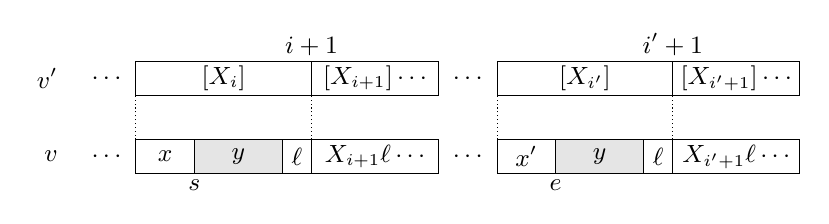
\begin{tikzpicture}[x=0.62cm,y=0.62cm,font=\small]
  % level j+1: the block word
  \node[anchor=east] at (-0.2,1.6) {$v'$};
  \node at (0.6,1.6) {$\cdots$};
  \draw (1.2,1.25) rectangle node{$[X_i]$} (4.8,1.95);
  \draw (4.8,1.25) rectangle node{$[X_{i+1}]\cdots$} (7.4,1.95);
  \node at (8.0,1.6) {$\cdots$};
  \draw (8.6,1.25) rectangle node{$[X_{i'}]$} (12.2,1.95);
  \draw (12.2,1.25) rectangle node{$[X_{i'+1}]\cdots$} (14.8,1.95);
  \node[above,inner sep=2pt] at (4.8,1.95) {$i+1$};
  \node[above,inner sep=2pt] at (12.2,1.95) {$i'+1$};
  % level j: the expansion
  \node[anchor=east] at (-0.2,0) {$v$};
  \node at (0.6,0) {$\cdots$};
  \draw (1.2,-0.35) rectangle node{$x$} (2.4,0.35);
  \draw[fill=black!10] (2.4,-0.35) rectangle node{$y$} (4.2,0.35);
  \draw (4.2,-0.35) rectangle node{$\ell$} (4.8,0.35);
  \draw (4.8,-0.35) rectangle node{$X_{i+1}\ell\cdots$} (7.4,0.35);
  \node at (8.0,0) {$\cdots$};
  \draw (8.6,-0.35) rectangle node{$x'$} (9.8,0.35);
  \draw[fill=black!10] (9.8,-0.35) rectangle node{$y$} (11.6,0.35);
  \draw (11.6,-0.35) rectangle node{$\ell$} (12.2,0.35);
  \draw (12.2,-0.35) rectangle node{$X_{i'+1}\ell\cdots$} (14.8,0.35);
  \node[below,inner sep=2pt] at (2.4,-0.35) {$s$};
  \node[below,inner sep=2pt] at (9.8,-0.35) {$e$};
  \draw[densely dotted] (4.8,0.35) -- (4.8,1.25);
  \draw[densely dotted] (12.2,0.35) -- (12.2,1.25);
  \draw[densely dotted] (1.2,0.35) -- (1.2,1.25);
  \draw[densely dotted] (8.6,0.35) -- (8.6,1.25);
\end{tikzpicture}
\caption{The alignment lemma. Bottom: a comparison $(s,e)$ of the expansion $v$
with $e<\len v$ starts in two blocks $X_i=xy$ and $X_{i'}=x'y$ that have the
common suffix $y$ (shaded) after $s$ and after $e$, so both cuts lie at the same
distance from the markers that close their blocks. Top: what follows these two
markers is the expansion of the block word $v'$ after the cuts $i+1$ and $i'+1$,
so $(s,e)$ is a comparison of $v$ iff, in addition, $(i+1,i'+1)$ is a
comparison of $v'$.}
\Description{Two rows. The top row is the block word with the letters X i,
X i plus one and so on, X i prime, and X i prime plus one and so on; the cuts
after X i and after X i prime are labeled i plus one and i prime plus one. The
bottom row is the expansion: each block X i is drawn as x followed by a shaded
y and the marker, and X i prime as x prime followed by a shaded y and the
marker. The cut s lies before the first shaded y, the cut e before the second.
Dotted lines connect each block of the top row to its expansion.}
\label{fig:bg-alignment}
\end{figure}

For example, the comparison $(0,6)$ of $w=01001101$, with $\wsuf w6=01$,
starts in the blocks $X_0=0$ and $X_3=0$ of $w=(0)1(00)1(\eps)1(0)1$, both at
distance one from their markers and with the common suffix $y=0$, and $(1,4)$ is
the terminal comparison of $w_1=[0][00][\eps][0]$ that ends at its last cut. A
comparison of one level thus reappears at the next level as a comparison of
blocks, together with a test at the same distance from the ends of two blocks.
The derivatives of lettered monitors (\cref{def:bg-derivative}) check
comparisons in exactly this form.

Depth measures how deeply such repetitions are nested. It matters because the
compression behind \cref{thm:bg-search} works one level of the hierarchy at a
time, so its length bound grows with the depth. The depth of a rejected word is
bounded in terms of its rejected tail, for every reader. The key step is the
following lemma.

\begin{lemma}[Return gap {\nssecite{Lemma ``Return gap''}}]\label{lem:bg-return-gap}
Let $w$ be a rejected word of a reader. If $(s,e)$ is a comparison of $w$ and
$q_s=q_e$, then $e-s\le r(w)$.
\end{lemma}
\begin{proof}
Put $\varpi=e-s$. The comparison gives $\wpre ws\,\wsuf we=\wpre w{\len
w-\varpi}$. Since $q_s=q_e$, reading $\wsuf we$ from $q_s$ ends in $q_{\len w}$,
so the state at the cut $\len w-\varpi$ is $q_{\len w}\in\Rej$. By minimality of
$J(w)$, $\len w-\varpi\ge J(w)$, so $\varpi\le r(w)$.
\end{proof}

\begin{theorem}[Depth from the rejected tail {\nssecite{Theorem ``Depth from tail''}}]\label{thm:bg-depth}
For every reader with $N$ states, every nonempty rejected word $w$
satisfies $\depth(w)\le2N(r(w)+1)-1$.
\end{theorem}

\begin{theorem}[Bounded-depth search {\nssecite{Theorem ``Bounded-depth search''}}]\label{thm:bg-search}
Let $(\mathcal M,\Adm,\Rej)$ be a reader with $N$ states over a finite alphabet,
and let $d\ge0$. If it has a nonempty hole of depth at most $d$, then it has a
nonempty hole of depth at most $d$ and length at most $\holeBound(N,d)$, the
explicit elementary function of \cref{eq:bg-len}. The same holds for every
lettered monitor with $N$ states over any alphabet (defined below,
\cref{def:bg-monitor}).
\end{theorem}

\Cref{thm:bg-depth} applies to every nonempty rejected word, whether or not it
is a hole, and neither theorem uses the rejected-path property or a property of
subtype constraints; the alphabet size does not enter the bounds. Combined with
\cref{thm:bg-brt}, they decide the hole problem for readers with the
rejected-path property.

\begin{corollary}[Finite search for holes {\nssecite{Theorem ``Finite search for holes'', Lemma ``Elementary estimate''}}]\label{cor:bg-hole-decision}
Let a reader with $N$ states over a finite alphabet have the rejected-path
property, and put $d_N=2N(4N-1)-1$. It has a hole iff it has a hole of length
at most $\holeBound(N,d_N)$, and $\holeBound(N,d_N)\le2^{2^{1280(N+1)^5}}$.
\end{corollary}
\begin{proof}
By \cref{thm:bg-brt}, some hole $w$ has $r(w)\le4N-2$. If $w$ is empty, it meets
the bound. Otherwise \cref{thm:bg-depth} gives $\depth(w)\le d_N$, and
\cref{thm:bg-search} gives a hole of length at most $\holeBound(N,d_N)$. The
converse is trivial, and the estimate is \cref{lem:bg-estimate}.
\end{proof}

\paragraph{Lettered monitors}
The proof of \cref{thm:bg-search} reads each level of the hierarchy of a hole
with its own automaton, obtained from the automaton of the level below by a
derivative. These automata evaluate their tests at positions inside blocks, so
the tests see the letters as well as the states.

\begin{definition}[Lettered monitor {\nssecite{Sect.\ ``Lettered Monitors and Their Derivatives''}}]\label{def:bg-monitor}
A \emph{lettered monitor} $\mathcal M$ over an alphabet $\Gamma$, possibly
infinite, has a finite state set $\mathcal Q$, a start state $\zeta_0$, a
transition function $\delta:\mathcal Q\times\Gamma\to\mathcal Q$, a
\emph{final-target} predicate $\Tfin\subseteq\mathcal Q\times\Gamma$, and two
relations $\Lambda$ and $\Lfin$ on \emph{labels}, the second for terminal
comparisons. Labels are a symbol $\triangleright$, the \emph{start label}, and
the pairs $(\zeta,a)\in\mathcal Q\times\Gamma$. Reading a word $v$ gives the
states $\zeta_{i+1}=\delta(\zeta_i,v[i])$ and the labels $L_0=\triangleright$
and $L_i=(\zeta_{i-1},v[i-1])$ for $1\le i\le\len v$. A nonempty word $v$ is a
\emph{hole} of $\mathcal M$ if $\Tfin(L_{\len v})$ holds, no terminal comparison
$(s,\len v)$ has $\Lfin(L_s,L_{\len v})$, and no other comparison $(s,e)$ has
$\Lambda(L_s,L_e)$.
\end{definition}

So the label of a cut $i\ge1$ is the last transition before it: the state at
the cut $i-1$ and the letter read from it. A reader $(\mathcal M,\Adm,\Rej)$
with states $Q$, start $q_0$, and transition $\delta$ determines the lettered
monitor with the same states and transitions, $\Tfin(\zeta,a)$ iff
$\delta(\zeta,a)\in\Rej$, and $\Lambda=\Lfin$ given by $\Adm$ on the
\emph{denoted} states, where $\den(\triangleright)=q_0$ and
$\den(\zeta,a)=\delta(\zeta,a)$. Since $\den(L_i)=q_i$, the reader and this
monitor have the same nonempty holes. The tests take labels, and not only the
states they denote, because the monitors of higher levels evaluate them at
positions inside blocks, which requires the letters.

\paragraph{Shifted blocks and derivatives}
Fix a marker $\ell\in\Gamma$, a block $X\in(\Gamma\setminus\{\ell\})^*$, and
$\zeta\in\mathcal Q\sqcup\{\star\}$, where $\star$ is a fresh symbol. The
\emph{shifted block} of $X$ read from $\zeta\in\mathcal Q$ is the word $\ell X$
read from $\zeta$; read from $\star$, it is $X$ read from $\zeta_0$. It has a
label $\lab_g(\zeta,X)$ at each position $g=0,\ldots,\len X$: for
$\zeta\in\mathcal Q$, the label of the cut after $\ell\,\wpre Xg$, so that
position $0$ carries the \emph{marker label} $(\zeta,\ell)$; for $\zeta=\star$,
the label $\triangleright$ at position $0$ and the label of the cut after
$\wpre Xg$ at positions $g\ge1$. The \emph{exit} $\delta_\ell(\zeta,X)\in\mathcal
Q$ is the state at the end of the shifted block. In a word of blocks read by
the derivative below, the \emph{entry state} of a position is the state at the
cut before it, from which the shifted block of its letter is read.

\begin{definition}[Derivative {\nssecite{Definition ``Derivative''}}]\label{def:bg-derivative}
The \emph{derivative} $\mathcal M_\ell$ of $\mathcal M$ along $\ell$ is the
lettered monitor over $(\Gamma\setminus\{\ell\})^*$ with states $\mathcal
Q\sqcup\{\star\}$, start state $\star$, transitions $\delta_\ell$, and
\[
\begin{aligned}
 \Lambda_\ell((\zeta,X),(\zeta',X'))&\iff X=xy,\ X'=x'y,\
   \Lambda\bigl(\lab_{\len x}(\zeta,X),\lab_{\len{x'}}(\zeta',X')\bigr)
   \text{ for some }x,x',y,\\
 \Lfin_\ell((\zeta,X),(\zeta',X'))&\iff \Lambda_\ell((\zeta,X),(\zeta',X'))
   \ \text{or}\ \Lfin\bigl(\lab_g(\zeta,X),(\delta_\ell(\zeta',X'),\ell)\bigr)
   \text{ for some }g\le\len X,\\
 \Tfin_\ell(\zeta,X)&\iff \Tfin(\delta_\ell(\zeta,X),\ell)\ \text{and}\
   \neg\Lfin\bigl(\lab_g(\zeta,X),(\delta_\ell(\zeta,X),\ell)\bigr)
   \text{ for all }g\le\len X;
\end{aligned}
\]
every relation with the start label $\triangleright$ of $\mathcal M_\ell$ as an
argument is false.
\end{definition}

In words: $\Lambda_\ell$ compares two positions at the same distance from the
ends of two blocks, with equal letters after them, as in
\cref{lem:bg-alignment}; the second disjunct of $\Lfin_\ell$ compares a position
anywhere in the block of its first argument with the final cut, which carries
the label of the closing marker; and $\Tfin_\ell$ checks the original target and
all terminal comparisons that start in the last block. Comparisons of the
expansion that start at its cut $0$ are represented inside the first shifted
block, whose entry is $\star$, so setting the relations at the new start label
to false discards none of them.

\paragraph{The label facts}
Let $v=X_0\ell X_1\ell\cdots X_{k-1}\ell$ be the expansion of a nonempty word
$v'=[X_0]\cdots[X_{k-1}]$ of blocks avoiding $\ell$. Let $\zeta'_0=\star$ and
$\zeta'_{i+1}=\delta_\ell(\zeta'_i,X_i)$ be the run of $v'$ in $\mathcal
M_\ell$, put $a_i=\len{X_0\ell\cdots X_{i-1}\ell}$, and let
$b_i=a_i+\len{X_i}$ be the position of the marker closing $X_i$. The intervals
$[a_i,b_i]$ partition the cuts $0,\ldots,\len v-1$, and the labels $L$ of $v$ in
$\mathcal M$ and $L'$ of $v'$ in $\mathcal M_\ell$ satisfy the \emph{label
facts} \nssecite{proof of Lemma ``Holes under desubstitution''}
\begin{equation}\label{eq:bg-label-facts}
 L_{a_i+g}=\lab_g(\zeta'_i,X_i)\quad(0\le g\le\len{X_i}),\qquad
 L_{\len v}=(\zeta'_k,\ell),\qquad
 L'_{i+1}=(\zeta'_i,X_i).
\end{equation}
In particular $\zeta'_{i+1}$ is the state of $\mathcal M$ at the cut $b_i$.

\begin{lemma}[Holes under desubstitution {\nssecite{Lemma ``Holes under desubstitution''}}]\label{lem:bg-desub}
With $v$ and $v'$ as above, $v$ is a hole of $\mathcal M$ iff $v'$ is a hole of
$\mathcal M_\ell$. Consequently, if $\mathcal M_0$ is a lettered monitor with $N$
states and $\mathcal M_{j+1}=(\mathcal M_j)_{\ell_j}$ along the canonical
hierarchy of a nonempty word $w$, then $w$ is a hole of $\mathcal M_0$ iff $w_j$
is a hole of $\mathcal M_j$, for every $j$, and $\mathcal M_j$ has $N+j$
states.
\end{lemma}

\begin{example}[A derivative]
Let a lettered monitor $\mathcal M$ over $\{0,1\}$ read $w=01001101$, with the
state $\zeta_h$ and the label $L_h$ at the cut $h$. With the marker $\ell=1$,
the next level $w_1=[0][00][\eps][0]$ has the blocks $X_0=0$, $X_1=00$,
$X_2=\eps$ and $X_3=0$, which begin at the cuts $0$, $2$, $5$ and $6$ of $w$:
\begin{center}
\small
\begin{tabular}{@{}ccccc@{}}
\toprule
$i$ & $X_i$ & cuts $a_i$--$b_i$ & entry $\zeta'_i$ & label $L'_{i+1}$\\
\midrule
$0$ & $0$ & $0$--$1$ & $\star$ & $(\star,0)$\\
$1$ & $00$ & $2$--$4$ & $\zeta_1$ & $(\zeta_1,00)$\\
$2$ & $\eps$ & $5$ & $\zeta_4$ & $(\zeta_4,\eps)$\\
$3$ & $0$ & $6$--$7$ & $\zeta_5$ & $(\zeta_5,0)$\\
\bottomrule
\end{tabular}
\end{center}
The marker is $1$, so $\mathcal M_1$ is both the derivative along $1$ and the
monitor of level $1$. By the label facts, the run of $w_1$ in $\mathcal M_1$ is
$\star,\zeta_1,\zeta_4,\zeta_5,\zeta_7$, the states before the four markers,
and the labels of $w_1$ are those in the last column; the shifted block of
$X_3$, for instance, is the factor $10$ of $w$ between the cuts $5$ and $7$.

The comparisons of $w_1$ that start after its cut $0$ are the terminal pairs
$(1,4)$, $(2,4)$ and $(3,4)$, which $\mathcal M_1$ tests with $\Lfin_1$. For
$(1,4)$, the first disjunct $\Lambda_1(L'_1,L'_4)$ takes the two common
suffixes $0$ and $\eps$ of $X_0$ and $X_3$ and reads $\Lambda(L_0,L_6)$ and
$\Lambda(L_1,L_7)$: the comparisons $(0,6)$ and $(1,7)$ of $w$
(\cref{fig:bg-alignment}). The second disjunct reads $\Lfin(L_0,L_8)$ and
$\Lfin(L_1,L_8)$: the terminal comparisons of $w$ that start in $X_0$. In the
same way, $(2,4)$ stands for the comparisons $(3,6)$ and $(4,7)$ and for the
terminal comparisons from the cuts $2$, $3$ and $4$, and $(3,4)$ for $(5,7)$
and the terminal comparison from the cut $5$. Finally, $\Tfin_1(L'_4)$ reads
the final target $\Tfin(L_8)$ and excludes the terminal comparisons from the
cuts $6$ and $7$, which start in the last block. These are all the comparisons
of $w$, so $w$ is a hole of $\mathcal M$ iff $w_1$ is a hole of $\mathcal M_1$.
The comparisons $(0,3)$ and $(0,4)$ of $w_1$ start at its start label, where
every relation of $\mathcal M_1$ is false.
\end{example}

\paragraph{How the bounded-depth search works}
Later sections extend the proof of \cref{thm:bg-search}, which has five steps;
\cref{app:bg-search} states them precisely. Let $w$ be a nonempty hole of depth
$D\le d$ with hierarchy $(w_j,\ell_j)$.
\begin{enumerate}[leftmargin=*]
\item \emph{Derivatives.} Let $\mathcal M_0$ be the lettered monitor of the
  reader, and $\mathcal M_{j+1}=(\mathcal M_j)_{\ell_j}$. By
  \cref{lem:bg-desub}, $w_j$ is a hole of $\mathcal M_j$ for every $j$. The
  $N+j$ states of $\mathcal M_j$ are the $N$ \emph{ordinary} states of
  $\mathcal M_0$ and the \emph{symbolic} start states $\star_1,\ldots,\star_j$
  added by the derivatives; ordinary states lead to ordinary states
  (\cref{app:bg-monitors}).
\item \emph{Dictionary normal form.} At each level $1\le i<D$, two isolated
  letters with the same exchange type are merged: the one with the longer
  expansion is replaced by the other, which keeps the comparisons and the
  state run of the level, and the level stays a hole
  (\cref{lem:bg-isolated-exchange}). The result is again a hole of depth $D$,
  no longer. Repeating this bounds the dictionary at every level
  $i\ge1$ by $\mathsf G(N,d)$. The terms are the following.
  \begin{description}[leftmargin=1em,font=\normalfont\itshape]
  \item[Dictionary.] The \emph{dictionary} of level $i$ is the set of letters
    of $w_i$.
  \item[Protected and unprotected letters.] The \emph{protected} letters of
    level $i$ are the marker $\ell_i$ and the letters of the \emph{start
    prefix}, the first at most $i$ positions of $w_i$, which are read from
    symbolic states; every other letter is \emph{unprotected} and is read only
    from ordinary states.
  \item[Isolated letters.] An unprotected letter is \emph{isolated} if all its
    unequal comparison partners are protected: whenever it precedes one cut of
    a comparison and a different letter precedes the other cut, that letter is
    protected.
  \item[Exchange type.] The \emph{exchange type} of an unprotected letter is
    the finite table of how $\mathcal M_i$ treats it when it is read from an
    ordinary state: its transitions and final targets, and the values of
    $\Lambda_i$ and $\Lfin_i$ when it is compared with itself (the \emph{self
    table}), with a protected letter (the \emph{protected rows}), and with the
    start label (the \emph{initial row}).
  \end{description}
\item \emph{The top level.} The unary top level $w_D$ is shortened to at most
  $N+D$ letters by keeping a prefix with the same last label
  (\cref{lem:bg-unary}).
\item \emph{Simultaneous compression.} Going down from the top, the at most
  $\mathsf G(N,d)$ distinct blocks in use at each level are written as the
  tracks of one word of \emph{columns}, aligned at their right ends, and
  shortened together by deleting the columns between two cuts with equal
  \emph{summaries}. The summary of a tuple of blocks records, for every entry
  state, the exit of each block and the final marker labels to which $\Lfin$
  relates its labels, which blocks are equal, and which pairs of blocks the
  derived admission relates; so it determines the derived monitor on the letters in use, and the
  shortened word is again a hole. Precisely, the new derived monitors
  \emph{agree} with the old ones on the letters in use, the \emph{support}: up
  to the renaming of each letter by its shortened version, they have the same
  states, transitions, targets and relations (\cref{eq:bg-agreement}). The
  induction that produces the new markers level by level from the top is the
  \emph{supported compression} of \cref{lem:bg-compression}.
\item \emph{The bound.} Each shortened block has fewer than
  $\mathsf{col}(N+d+1,\mathsf G(N,d))$ letters, so each of the at most $d$
  expansions multiplies the length by at most this factor. With the top level
  this gives $\holeBound(N,d)$.
\end{enumerate}
Shortening each block separately would fail, because comparisons relate
different blocks through equal suffixes. The compression keeps a word a hole,
that is, it preserves the absence of admitted comparisons, but it may destroy
any particular comparison; positive conditions need the extension of
\cref{sec:mo}.
